\section{Introduction}
\label{sec:intro}

%\paragraph{Motivation}
Computing statistical properties of 
complex systems containing uncertain parameters is
challening due to the need for a large number of expensive model evaluations. 
Surrogate models make such computations possible by replacing 
expensive model runs with cheap evaluations of an approximate model.
%
%Surrogate modeling has become a critical component of scientific computing
%owing to the emergence of the field of uncertainty quantification for
%scientific and engineering applications. 
%
Commonly used approaches for surrogate modeling include polynomial chaos
expansions (PCEs)~\cite{Xiu:2002,Ghanem:2003,Olivier:2010}, multivariate
adaptive regression splines (MARS)~\cite{friedman93}, Gaussian processes
(GPs)~\cite{Rasmussen:2004}, or Kriging~\cite{Stein:2012}. A pertinent
challenge associated with surrogate construction involves the process of
\textit{training} that typically requires a large number of model runs.  In
situations involving large-dimensional systems, and computationally intensive
simulations, the training of a surrogate becomes challenging and
even prohibitive in some cases. A possible approach for mitigating this
challenge involves computation of global sensitivity measures such as Sobol'
indices~\cite{Sobol93,Sobol:2001,Owen13,SaltelliRattoAndresEtAl08} to identify
the \emph{important parameters}---i.e., parameters that predominantly
contribute towards the variability of the model output. 

Sensitivity-based
dimension reduction can help reduce the computational effort
significantly. However, numerically estimating the Sobol' indices, which
involve multi-dimensional integrals, can be a demanding task in itself. In
fact, often surrogate models are constructed to estimate the Sobol' sensitivity
indices; this has been done for a variety of applications including in ocean
modeling~\cite{AlexanderianWinokurSrajEtAl12,LiIskandaraniLeHenaffEtAl16},
geosciences~\cite{Namhata2016OladyshkinDilmoreEtAl16,deman2016,SaadAlexanderianPrudhommeEtAl17},
and chemical kinetics~\cite{DegasperiGilmore08,navarro2016global,Vohra:2014} to
name a few. 
We are thus, faced with a ``chicken-and-egg'' problem: on the one hand,
computing global sensitivity measures enable dimension reduction, which in turn
enable efficient surrogate model construction.  On the other hand, computing
sensitivity measures is expensive and is often made possible by using
surrogate models. Development of an approach for 
overcoming this chicken-and-egg problem is a major goal of this article. 

 
%Hence, this common practical issue in scientific computing can
%be characterized as a ``chicken-and-egg" problem. 

In this article, we propose a practical and efficient approach that focuses on
optimal use of computational resources for surrogate construction in a 
reduced-input space. Specifically, we reduce the dimensionality of the
input space by using the derivative-based global sensitivity
analysis~\cite{Sobol:2009,Sobol:2010,Lamboni:2013,Kucherenko:2009,Kucherenko:2016},
which enables a tractable approach for global sensitivity
analysis~\cite{Kucherenko:2016}. The links between derivative based
global sensitivity measures (DGSMs) and total Sobol'
indices~\cite{Sobol:2009,Kucherenko:2009,Kucherenko:2016} provide a strong
basis for their use in identifying unimportant parameters. In addition
to the construction of an efficient surrogate in the reduced space,
dimension reduction highlights key features of the input-output relationship
encapsulated by the model, and allows for an efficient approach to calibration
of the important inputs. 

%The emerging field of uncertainty quantification (UQ) aims at methodologies for
%incorporating, characterizing, quantifying, propagating, and reducing the
%uncertainties associated with predictive models and simulations.  For
%situations involving complex physical models and computationally intensive
%simulations, surrogate modeling often provides orders of magnitude speedups in
%statistical studies. This is done by replacing repeated evaluations of
%computationally expensive models by inexpensive evaluations of a surrogate
%model.  Thus, an efficient approach to construction of surrogate models is of
%central importance in enabling efficient uncertainty quantification for
%computationally intensive models. 
%
%
%Commonly used surrogate modeling approaches use polynomial chaos expansions
%(PCEs)~\cite{Xiu:2002,Ghanem:2003,Olivier:2010}, multivariate adaptive
%regression splines (MARS)~\cite{friedman93}, Gaussian processes
%(GPs)~\cite{Rasmussen:2004}, or Kriging~\cite{Stein:2012}.  Many real-world
%applications involve a large number of model inputs. This makes
%the construction of surrogate models difficult or impossible in some cases.
%However, in many situations, the variability in model observables of interest
%is sensitive to only a small subset of the uncertain inputs.  Hence,
%identifying model inputs that are inessential to variability in model output is
%a key step that can help reduce the input parameter dimension and hence the effort
%associated with surrogate model construction. 

%However, both approaches
%quickly become prohibitive when the set of uncertain model inputs and
%parameters is large-dimensional. Specifically, in the case of a PCE, a
%$d$-dimensional polynomial basis with a total order of truncation, $p$ requires
%model realizations at $(p+1)^d$ quadrature nodes to exactly determine the PC
%coefficients using a fully-tensorized Gauss quadrature. Consider a case where
%$d$ = 8 which could be a regarded as a low-dimensional problem, and $p$ = 5,
%requires model evaluations at roughly 1.7 million quadrature nodes. However,
%the degree of exactness in numerical estimation of the coefficients as made
%%possible with a fully-tensored quadrature might not be desired. In that case,
%computational effort can be reduced considerably by using nested
%quadratures~\cite{Gentleman:1972a,Gentleman:1972b,Novak:1999,Waldvogel:2006}
%%which allow model realizations at a given level to be used at higher levels of
%accuracy as well as sparse grids based on Smolyak
%tensorization~\cite{Smolyak:1963}. Additionally, sparse basis
%techniques~\cite{Peng:2014,Hampton:2015,Blatman:2011} have been used to reduce
%the required computational effort for constructing a reasonably accurate PC
%surrogate. 

%One of the primary objectives for constructing a model surrogate is to be able
%to perform parametric sensitivity analysis tractably. 

%Variance based global sensitivity analysis based on Sobol' indices~\cite{Sobol93,
%Sobol:2001,Owen13,SaltelliRattoAndresEtAl08} provides
%insight into the relative contributions of the uncertain model inputs to the
%uncertainty in predictions. Specifically, such analysis can help reduce the
%dimensionality of the problem.  Computing Sobol' indices, however, is a
%computationally demanding task.  
%Availability of a surrogate model typically
%enables efficient computation 
%of Sobol' indices~\cite{Sudret08,CrestauxLeMaitreMartinez09,BlatmanSudret10,HartAlexanderianGremaud17,Sargsyan17}. This has enabled performing global sensitivity analysis
%on a wide range of applications including in ocean 
%modeling~\cite{AlexanderianWinokurSrajEtAl12,LiIskandaraniLeHenaffEtAl16},
%geosciences~\cite{Namhata2016OladyshkinDilmoreEtAl16,deman2016,SaadAlexanderianPrudhommeEtAl17},
%and chemical kinetics~\cite{DegasperiGilmore08,navarro2016global,Vohra:2014}
%to name a few.
%
%While surrogate models provide an efficient way of computing sensitivity
%indices, constructing them in the case of models with high-dimensional inputs
%can be as expensive as computing the Sobol' indices via sampling. 
%In this article, we propose a practical and efficient
%approach to address this commonly observed ``chicken-and-egg'' problem
%in surrogate modelling for engineering applications.
%Specifically, we reduce
%the dimensionality of the input space using derivative-based global sensitivity
%analysis~\cite{Sobol:2009,Sobol:2010,Lamboni:2013,Kucherenko:2009,Kucherenko:2016},
%which enables a tractable approach for global sensitivity
%analysis~\cite{Kucherenko:2016}. The links between derivative based
%global sensitivity measures (DGSMs) and total Sobol'
%indices~\cite{Sobol:2009,Kucherenko:2009,Kucherenko:2016} provide a strong
%basis for their use in identifying unimportant parameters. In addition
%to the construction of an efficient surrogate in the reduced space,
%dimension reduction highlights key features of the input-output relationship
%encapsulated by the model, and allows for an efficient approach to calibration
%of the important inputs. 


%However, as discussed
%earlier, constructing the surrogate might still require a large amount of
%computational resources. 


\paragraph{Our approach}
We present a strategy for identifying and screening uncertain model parameters
that are significantly less important than the rest, thereby reducing the
dimensionality of the problem and enabling the construction of a reduced-space
surrogate (RSS).  Our approach combines DGSMs and surrogate modeling in an
iterative manner.  To make optimum use of computational resources, batches of
model evaluations are performed iteratively, and convergence of our DGSM based
screening metric is tested successively. Moreover, a series of verification steps
incorporated in our method enable monitoring the accuracy of the parameter-screening
and the resulting surrogate model.  Our approach is agnostic to the choice of
methodology for constructing the surrogate. However, in the present work, we
rely on sparse polynomial chaos expansions (PCEs) 
to demonstrate the suitability of the proposed strategy.  

%Moreover, the availability of adjoint solvers for
%efficient gradient computation can enhance the performance of our approach.  


\paragraph{Contributions}
The contributions of this article are as follows: (i) We establish a robust and
practical framework for dimension reduction and surrogate modeling using
derivative-based global sensitivity measures. Our
approach is general in that it is applicable to a wide range of applications.
(ii) We present comprehensive numerical results demonstrating the viability of
our strategy using motivating applications: the classic borehole
function, and a semilinear elliptic PDE.  (iii) We 
deploy our strategy in an application problem from chemical kinetics with 19
uncertain parameters. The problem is studied in multiple regimes.
It is shown that the 19-parameter problem can be efficiently reduced to a 3- 
or 4-dimensional problem.

\paragraph{Paper outline}
This article is structured as follows. In section~\ref{sec:bg}, we provide a
brief introduction to DGSMs as well as the polynomial chaos methodology used in
the present work.  In section~\ref{sec:method}, we present our proposed
approach, where we also provide a detailed numerical algorithm and a flow
diagram to aid practitioners in implementing the presented framework.
Section~\ref{sec:examples} is devoted to numerical examples
examining various aspects of our approach. This is followed by implementation
of our framework in a H$_2$/O$_2$ chemical kinetics problem, in section~\ref{sec:app}.
Finally, concluding remarks are provided in section~\ref{sec:disc}.


%\begin{figure}[htbp]
% \begin{center}
%  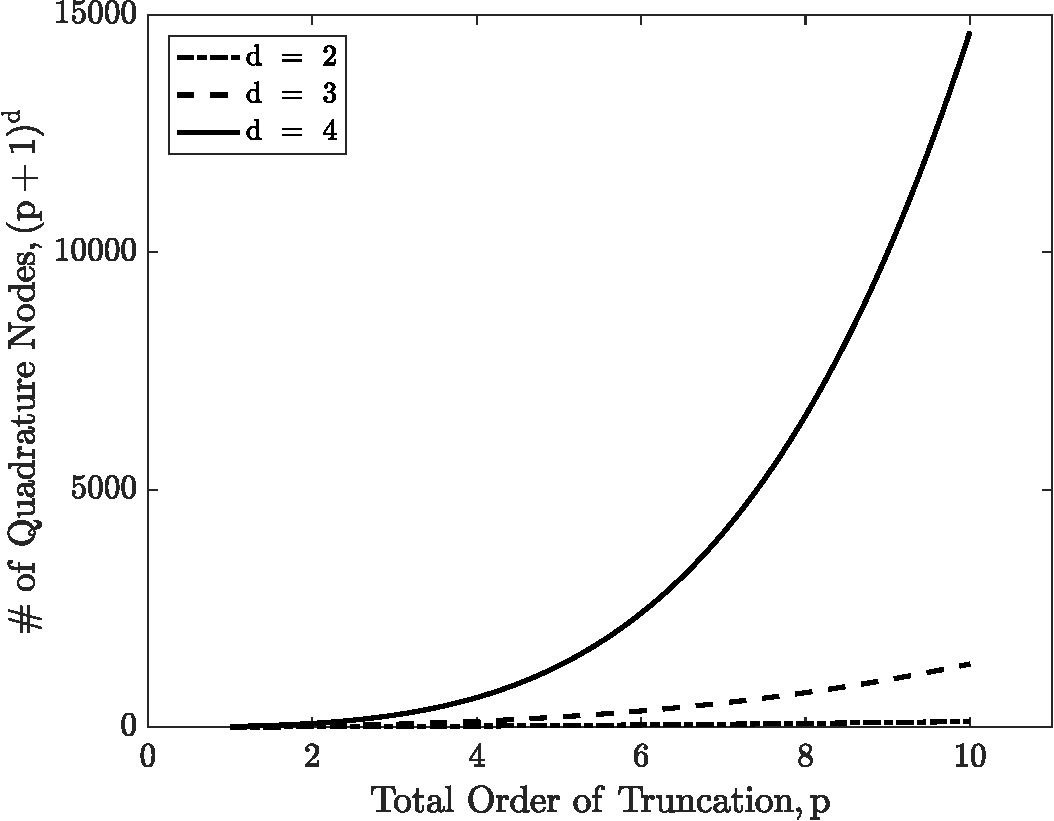
\includegraphics[width=0.70\textwidth]{./Figures/curse}
%\caption{Number of multi-dimensional Gauss quadrature nodes, $(p+1)^d$ is plotted against the PCE
% total order truncation, $p$ for 2, 3, and 4 dimensional polynomial basis functions.}
%\label{fig:curse}
%\end{center}
%\end{figure}




